\documentclass[a4paper,11pt]{article}

\usepackage{exptech,hyperref}
\hypersetup{
	colorlinks=true,                         
	citecolor=black, % Couleur des numéros de la biblio dans le corps
	urlcolor=blue,   % Couleur des url
	linkcolor=black}  % Couleur des liens internes

%Décommanter pour la relecture (interlignes plus importantes)
%\linespread{1,6}

%%%%%%%%%%%%%%%%%%%%%%%%%%%%%%%%%%%%%%%%%%%%%%%%%%%%%%%%%%%%%%%%%%%%%%%%%%%%%%%

\title{ \textbf{Création d'un modèle 3D à partir de dessins 2D Documentation Technique} }
% Pour avoir le titre de l'expose sur chaque page

\author{ Aurélien \textsc{FONTAINE} Etienne \textsc{GEANTET} \\
	Manutea \textsc{HUANG} Arnaud \textsc{MARTIN} \\
	\\
	Encadrants : François \textsc{LEHERICEY}	Bertrand \textsc{COUASNON}}

\date{4 Mai 2015}                    % Ne pas modifier

%%%%%%%%%%%%%%%%%%%%%%%%%%%%%%%%%%%%%%%%%%%%%%%%%%%%%%%%%%%%%%%%%%%%%%%%%%%%%%%

\begin{document}

\maketitle                 % Génère le titre
\thispagestyle{empty}      % Supprime le numéro de page sur la 1re page

\begin{abstract}
	Notre projet fonctionne sous Unity 4.6.1 en mode éditeur, dû à des parties qui seront détaillées dans la partie du code de l'extrusion.
\end{abstract}

\section{arborescence}
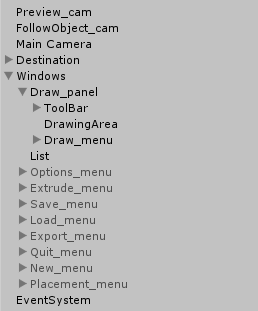
\includegraphics[scale=0.7]{./images/arborescence.png}
		\begin{itemize}
			\item Les trois premiers objets sont les caméras
				\begin{itemize}
					\item Preview\_cam est la caméra qui affiche en permanence en haut à droite le rendu de notre figure
					\item Follow\_ object est la caméra qui suis notre objets quand on le place dans l'environnement 3D
					\item Main camera est la caméra principale
				\end{itemize}
			\item Destination, c'est le contenant de tout les objets que l'ont va crée, c'est lui qui sera transmis par la suite au serveur. Il possède un sous item invisible, car cela posais des problèmes pour la disposition des caméras quand il n'y avais rien. Nous n'avons pas trouver d'où cela venais
			\item Windows, le canvas principal, c'est lui qui est filmé par la Main Camera
			\item Toolbar, barre de menu grise en haut
			\item DrawingArea, zone où l'on dessine
			\item Draw\_menu, menu des outils, il est associé à une animation pour la rentrée/sortie
			\item List, canvas vide qui représente la zone en bas à droite
			\item XXX\_menu, toutes les fenêtres
			\item Placement\_menu, ne suis pas le même modèle que les menus précédant, c'est ce qui permet le placement de la figure dans l'environnement 3D
		\end{itemize}
		
\section{Réseau}
	\subsection{Serveur}
		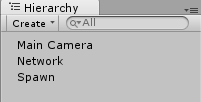
\includegraphics[scale=0.9]{./images/arbserver.png}
		\begin{itemize}
			\item Network contient le script qui gère la création et le comportement du serveur.
			\item Spawn est le point de repère pour faire apparaître l'objet reçu.
		\end{itemize}
		
		Le serveur se lance automatiquement au démarrage de l'application si Spawn et Network ne sont pas masqués.
		\subsubsection{Network et TcpServer}
			Le GameObject Network ne contient que le script "TcpServer".
			
			Le script "TcpServer" est composé essentiellement de 5 fonctions:
			\begin{itemize}
				\item Start : Crée un TcpListener et lance l'attente d'un client dans un thread qui tournera en arrière-plan.
				
				\item ListenForClients : Lance le TcpListener et attend qu'un client se connecte. Dès qu'un client est connecté, la communication avec ce client est établie dans un nouveau thread qui tournera en arrière-plan.
				
				\item HandleClientComm : Gère la communication avec le client. Tout d'abord nous créons un TcpClient chez le serveur, nous établissons un flux de données NetworkStream, et un buffer d'octets qui stocke 1Ko de données. Nous ne savons pas quelle sera la taille de l'objet donc nous écrivons progressivement dans un MemoryStream Ko par Ko en utilisant le buffer.
				Une fois que les données sont reçus, nous écrivons les données dans un fichier .prefab et nous fermons le fichier et le TcpClient.
				
				\item IsFileLocked : Rend vrai si le fichier est actuellement utilisé par une autre source. Faux sinon. Le fichier ne doit pas être bloqué pour pouvoir l'afficher.
				
				\item Appear : Fait apparaître l'objet au point de repère Spawn, cette fonction est utilisée dans Update, uniquement si le prefab peut-être utilisé, signalé par okPrefab.
			\end{itemize}
			
		\subsubsection{Adaptation}
			Pour importer le serveur sur une autre scène ou un autre projet Unity, il suffit de copier le script "TcpServer", de l'appliquer à un GameObject et de renseigner le GameObject repère pour l'apparition.
		
	\subsection{Client}

\end{document}